%%%%%%%%%%%%%%%%%%%%%%%%%%%%%%%%%%%%%%%%%%%%%%%%%%%%%%%%%%%%%%%%%%%%%%%%%%%%%%%%
%% MASTER'S THESIS                                                            %%
%%                                                                            %% 
%% Title (en): Mining Parallel Corpora from the Web                           %%
%% Title (sk): Rafinácia paralelných korpusov z webu                          %%
%%                                                                            %%
%% Author: Bc. Jakub Kúdela                                                   %%
%% Supervisor: Doc. RNDr. Irena Holubová, Ph.D.                               %%
%% Consultant: RNDr. Ondřej Bojar, Ph.D.                                      %%
%%                                                                            %%
%% Academic year: 2015/2016                                                   %%
%%%%%%%%%%%%%%%%%%%%%%%%%%%%%%%%%%%%%%%%%%%%%%%%%%%%%%%%%%%%%%%%%%%%%%%%%%%%%%%%

\chapter{Background Work and Prerequisities}
\label{chapter:background_work_and_prerequisities}

This chapter is an introduction to the resources and tools used in our work. It describes their features and properties and discusses their usefulness in our method or experiments. Before we introduce these individual resources and tools, let us first provide the context in which they are used by outlining the idea behind our method.

\section{Overview of Proposed Method}
\label{section:overview_of_proposed_method}

All the methods described in Chapter~\ref{chapter:related_work} operate on common basic principles. They assume the parallel data are most often created in the form of complete web pages with a similar HTML structure or matching URL, and they work well under these circumstances. However, we believe that there still exists a non-negligible amount of parallel data spread across the web pages that have different HTML structure and URL. Also, the order of corresponding segments may vary in different language versions of the same page. Moreover, some parallel content can be a part of a single web page. We would like to address all these situations.

The majority of described methods start the process by identifying candidate pairs of parallel web pages to be inspected. If a candidate pair has a similar HTML structure then the segments of the two web pages are aligned according to the structure. 

In contrast to these methods, our approach is more generic. The method considers as the input a set of plain text documents for both the languages. These can be all the paragraphs from a bilingual web domain. The intention is to identify candidate pairs of parallel documents. The problem is that for a given web domain, the number of possible pairs of paragraphs is usually significantly greater than the number of possible pairs of web pages. We have to reduce the number of candidate pairs of documents to be inspected as much as possible. Our method is supervised, and in order to be trained, it requires a sentence-aligned training parallel corpus for the given language pair. It begins by learning distributed word representations, i.e.\ word vectors, for both languages using the training corpus. These word vectors are similar for context-related words, even cross-lingually. They are used to calculate aggregate document vectors. Two parallel documents have a similar document vector. The document vectors for one language are subsequently hashed, forming a search index in such a way that similar vectors end up close to each other. The search index is then queried to obtain a short list of candidates for each document in the other language. At this stage, the complexity of the problem is significantly reduced. The method inspects the candidates to determine the best one using a bilingual dictionary. The bilingual dictionary is pre-calculated statistically using the training parallel corpus. This corpus is also used to train the binary classifier, that decides, at the end of the process, whether the pair consisting of a document and its top candidate should be considered parallel or not.

With the basic idea behind the method explained, let us describe the set of resources and tools we use in our work. The details of our method are elaborated in the next chapter.

\section{CzEng 1.0}
\label{section:czeng}

CzEng 1.0~\cite{Bojar12_2} is the fourth release of a sentence-aligned Czech--English parallel corpus, freely available for non-commercial research purposes. It consists of approximately 15 million sentence pairs (233 million English and 206 million Czech tokens) from seven different types of sources. The proportion of these source domains is summarized in Table~\ref{table:czeng}.

To download CzEng 1.0, one must first apply for the registration\footnote{\url{http://ufal.mff.cuni.cz/czeng} (accessed April 5, 2016)}. The corpus can be downloaded in multiple formats. In our experiments, we use all training sections (packs 00--97) of CzEng 1.0 in the plain text, untokenized format. A file in this format contains tab-separated values, where every line stands for a different sentence pair and individual columns represent:

\begin{enumerate}[itemsep=0pt]
	\item Sentence pair ID;
	\item Filter score (indicating the quality of the sentence pair);
	\item Czech sentence (untokenized);
	\item English sentence (untokenized).
\end{enumerate}

Because our method is supervised, it needs a sentence-aligned parallel corpus in order to be trained. For this purpose, we use CzEng 1.0 in our experiments. In one of them, we also utilize the alignment of the corpus to perform the evaluation of the method's efficiency. It is important to note that when using CzEng 1.0 as both the training and testing dataset, we first split the data into two equally sized parts: \textit{head} and \textit{tail}. The head is used for training, while the tail is used for evaluation. The domains are not grouped together within the corpus, but they are shuffled. This means that both head and tail should contain data from each domain.

\begin{table}[!htb]
	\centering
	\caption{CzEng 1.0 source domains distribution (Source:~\cite{Bojar12_2})}
	\label{table:czeng}
	\vspace{1em}
	\begin{tabular}{|l|r|r|}
		\hline
		\textbf{Source Domain} & \textbf{Sentences} & \textbf{Ratio (\%)} \\
		\hline
		Fiction & 4,335,183 & 28.64 \\
		EU Legislation & 3,992,551 & 26.38 \\
		Movie Subtitles & 3,076,887 & 20.33 \\
		Parallel Web Pages & 1,883,804 & 12.45 \\
		Technical Documentation & 1,613,297 & 10.66 \\
		News & 201,103 & 1.33 \\
		Project Navajo & 33,301 & 0.22 \\
		\hline
		\textbf{Total} & 15,136,126 & 100.00 \\
		\hline
	\end{tabular}
\end{table}

\section{MorphoDiTa}
\label{section:morphodita}

MorphoDiTa~\cite{Strakova14}\cite{Spoustova09} (Morphological Dictionary and Tagger) is an open-source tool performing morphological analysis of natural language texts. Its features include morphological analysis, morphological generation, tagging, and tokenization. It can be used either as a standalone tool or a library. 

In our experiment, we want to determine whether lemmatization helps our method get better quality results. For these purposes, we use MorpohoDiTa. As our experiments cover only the texts from the Czech--English language pair, we use available MorphoDiTa models for both Czech~\cite{Straka13} and English~\cite{Straka14}.

\section{SyMGIZA++}
\label{section:symgiza}

SyMGIZA++~\cite{Junczys10} is a tool for computing symmetric word alignment models. It is an extension of MGIZA++, which in turn is a successor of the historically original program called GIZA++.

GIZA++ is an implementation of the IBM Models 1--5~\cite{Brown93}, the HMM model~\cite{Vogel96}, and the Model 6~\cite{Och03}. Comparison of all these models was already analysed and discussed~\cite{Och03}. In the alignment process, it uses an Expectation–Maximization~\cite{Dempster77} (EM) algorithm. This iterative algorithm consists of two steps that are performed in each iteration. In the first step, called the E-step (expectation step), the previously computed model (or the initial model) is applied to the data and expected counts for individual parameters are computed using the probabilities of this model. The second step, called the M-step (maximization step), then takes these expected counts as a fact and uses them to estimate the probabilities of the next model. Furthermore, prior to the training itself, GIZA++ uses the program called mkcls~\cite{Och99} to create word classes. The notion of these classes helps in the training process.

GIZA++ was designed as a single-threaded application. However, MGIZA++~\cite{Gao08} extends GIZA++ with capabilities to run the alignment process in multiple threads on a single computer. This helps the overall speed of the program and reduces the time needed to accomplish the task.

All the models provided by the original GIZA++ are asymmetric. For a chosen translation direction, they allow words to be mapped in a many-to-one, but not in a one-to-many relationship. It is, therefore, quite common and popular to train models for both translation directions and symmetrize the resulting word alignments to allow more natural relationships between words. In this scenario, models for both directions are trained independently and post-symmetrization is applied as the final step of the process. However, the authors of SyMGIZA++ argue that introducing continuous symmetrization, during the whole training process, results in a better quality alignment. Unlike its predecessors, SyMGIZA++ produces results of the symmetrized models. Moreover, it allows us to update these symmetrized models between each iteration of the original training algorithms. The general training scheme,  depicted in Figure~\ref{figure:symgiza}, illustrates all the moments when the model parameters are combined during the process.

\begin{figure}[!htb]
	\centering
	\caption{General training scheme for SyMGIZA++ (Source:~\cite{Junczys10})}
	\label{figure:symgiza}
	\vspace{1em}
	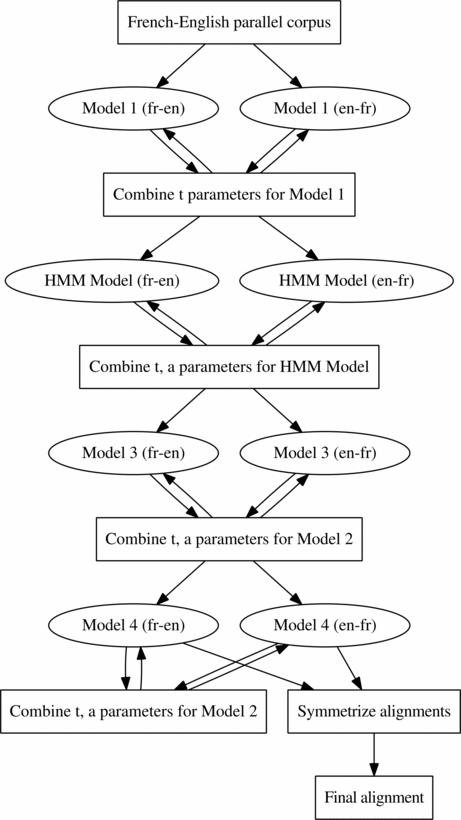
\includegraphics[width=0.6\textwidth]{images/symgiza.png}
\end{figure}

From all the available word aligning tools, such as GIZA++, MGIZA++, fast\_align~\cite{Dyer13}, etc., we decided to use SyMGIZA++. The results presented by its authors provide a convincing argument. They claim that the quality of the resulting alignment is increased by more than $17\%$ when compared to MGIZA++ or GIZA++, probably the most popular word alignment programs nowadays.

To train bilingual word vectors we need a parallel corpus together with its word alignment. In order to get the word alignment for the provided training corpus, we use SyMGIZA++. Furthermore, when running SyMGIZA++, the user can request the final values of the IBM Model 1 ``t'' parameters for both directions. In our method, these values are used to build the bilingual dictionary.

\section{bivec}
\label{section:bivec}

\textit{Word embedding} is a common name for a set of techniques which map words or phrases from a vocabulary to distributed word representations in the form of vectors consisting of real numbers in a high-dimensional continuous space. This section discusses bivec~\cite{Luong15}, a word embedding tool that creates bilingual word representations when provided with a word-aligned parallel corpus. The work is an extension of previous research, which resulted in a tool called word2vec~\cite{Mikolov13a}\cite{Mikolov13b}\cite{Mikolov13c}.

The original word2vec is a group of models producing monolingual word embeddings. These models are implemented as neural networks. They are trained to reconstruct the contexts of words. A monolingual corpus is needed for the training. During the training process, the algorithm iterates over the words in the corpus while considering the context of the current word in the form of a fixed-size window on its surrounding words. The two included models are:

\vbox{
\begin{itemize}
	\item The \textit{Continuous Bag-of-Words (CBOW)} model, trained to predict the word when given its context (without the current word).
	\item The \textit{Skip-gram (SG)} model, trained to predict the context of a given word.
\end{itemize}
}

\begin{figure}[!htb]
	\centering
	\caption{Continuous Bag-of-Words model (Source:~\cite{Rong14})}
	\label{figure:word2vec_cbow}
	\vspace{1em}
	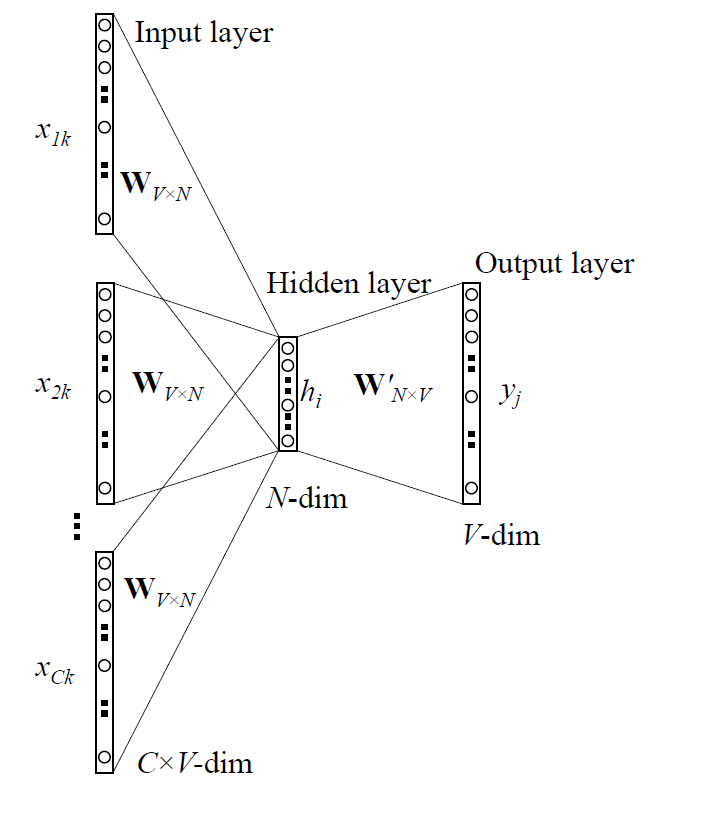
\includegraphics[width=0.6\textwidth]{images/word2vec_cbow.png}
\end{figure}

\begin{figure}[!htb]
	\centering
	\caption{Skip-gram model (Source:~\cite{Rong14})}
	\label{figure:word2vec_sg}
	\vspace{1em}
	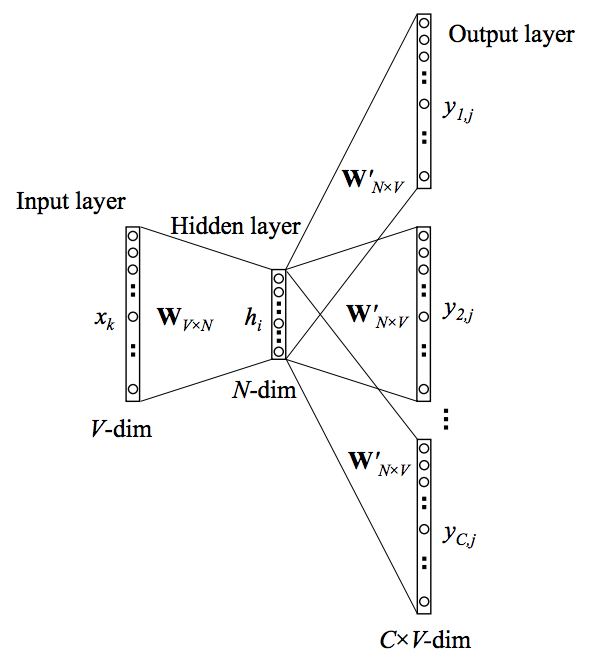
\includegraphics[width=0.6\textwidth]{images/word2vec_sg.png}
\end{figure}

The main difference between these two models can be observed in Figure~\ref{figure:word2vec_cbow} and Figure~\ref{figure:word2vec_sg}, which illustrate the structures of their underlying neural networks. When working with these networks, all the words are encoded to so-called one-hot vectors. This means that if $w_0, w_1, \ldots, w_V$ are all the unique words of the training corpus, word $w_i$ is encoded to a $V$-dimensional vector, where the $i$-th element is $1$ and all other $0$s.

In Figure~\ref{figure:word2vec_cbow}, one can see the one-hot vectors $x_{1,k}, x_{2,k}, \ldots, x_{C,k}$, representing the context of the current word in the input layer. In this model, the output layer consists of the one-hot vector of the word, $y_j$. On the other hand, Figure~\ref{figure:word2vec_sg} displays the one-hot vector of the word $x_k$ in the input layer, while the output layer contains the one-hot vectors of the words in its context, $y_{1,j}, y_{2,j}, \ldots, y_{C,j}$. In both these models, the user can choose the dimension of the hidden layer $N$ and the size of the context $C$. After the model is trained, it is used to map each of the words in the corpus to a vector. This vector is obtained from the hidden layer of the network and it represents the word's relationship with other words. The more the two words $w_i$, $w_j$ appear in the same context, the larger the \textit{cosine similarity} of their vectors $\operatorname{vec}(w_i)$, $\operatorname{vec}(w_j)$ is. Given two vectors $x$ and $y$, the cosine similarity is calculated as follows:

\begin{align*}
\operatorname{cos}(\textbf{x}, \textbf{y})=\frac{\textbf{x}\times\textbf{y}}{\lVert\textbf{x}\rVert\lVert\textbf{y}\rVert}= 
\frac{\sum\limits_{i=1}^{n} \textbf{x}_i\textbf{y}_i}{\sqrt{\sum\limits_{i=1}^{n} \textbf{x}_i^2} \sqrt{\sum\limits_{i=1}^{n} \textbf{y}_i^2}}.
\end{align*}

Word vectors obtained by training word2vec models have several interesting features. The relationship among the words are projected onto their vectors to such an extent, that for example the most similar vector to the resulting vector of an operation $\operatorname{vec}(\text{``king''}) - \operatorname{vec}(\text{``man''}) + \operatorname{vec}(\text{``woman''})$ is the vector $\operatorname{vec}(\text{``queen''})$. We will not pay further attention to more details about the advanced features of the word2vec results as they are not used in our method. It is worth mentioning that there are other related tools to word2vec, like for example GloVe~\cite{Pennigton14}.

The authors of bivec proposed an extension of the original Skip-gram model in the form of a joint bilingual model called the \textit{Bilingual Skip-gram (BiSkip)} model. When trained, this model can predict the context of a given word in both languages. In order to train, bivec requires a sentence-aligned parallel corpus and its word alignment. In fact, the word alignment is not strictly necessary, and if it is not provided, the system uses a simple heuristic. However, with the alignment provided, the results are better.

The most important idea behind the BiSkip model is the method of training. To gain insight into how the training works, let us look at the example illustrated in Figure~\ref{figure:bivec_bsg}. Suppose that we have two parallel sentences with their word alignment that says the English word ``trade'' is aligned with the German word ``Handels-''. We can use the associated German word ``Handels-'' to predict the surrounding English context containing the words like ``economic'' and ``financial''. Generally speaking, given a word $w_1$ in a language $l_1$, and a word $w_2$ in a language $l_2$ aligned to $w_1$, the BiSkip model uses the word $w_1$ to predict not only its own context in $l_1$, but also the context of the word $w_2$ in $l_2$. The other word $w_2$ is handled analogously. This results in training of a single Skip-gram model with a joint vocabulary on parallel corpora. In other words, BiSkip model is like a single Skip-gram model trained jointly to predict words for each of the language pairs $l_1 \rightarrow l_1$, $l_1 \rightarrow l_2$, $l_2 \rightarrow l_1$, and $l_2 \rightarrow l_2$ simultaneously. The resulting vector representations have the same properties, except that in this case they appear not only monolingually but also cross-lingually. It means, for example, that given a big enough English--German parallel corpus, the resulting vector representations of the words ``car'' and ``Auto'' would have greater cosine similarity.

\begin{figure}[!htb]
	\centering
	\caption{Bilingual Skip-gram model (Source:~\cite{Luong15})}
	\label{figure:bivec_bsg}
	\vspace{1em}
	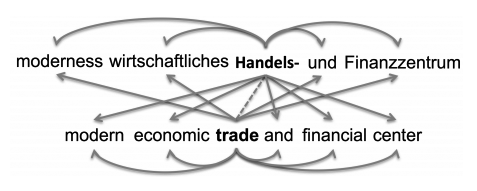
\includegraphics[width=0.6\textwidth]{images/bivec_bsg.png}
\end{figure}

Similarly to word2vec being not the only one among the monolingual word embedding strategies, bivec also has some interesting relatives. We could mention BilBOWA~\cite{Gouws14} (Bilingual Bag-of-Words without Alignments), a simple and computationally efficient model, which also learns bilingual distributed representations of words. The method does not require word alignment; instead, it trains directly on monolingual data using extracted bilingual signal from a potentially smaller sentence-aligned parallel corpus.

We decided to use bivec for learning the bilingual word vectors from the training parallel corpus. The results conducted by the authors suggest that bivec achieved state-of-the-art results among other similar approaches when applied in the field of cross-lingual document classification. Using the trained bilingual word vectors and the proper weighting scheme, our method calculates the aggregate document vectors. The similarities among the word vectors are reflected in the document vectors; therefore, a pair of parallel documents have similar vectors.

\section{Annoy}
\label{section:annoy}

Annoy~\cite{annoy} is a C++ library with Python bindings implementing the \textit{approximate-nearest-neighbors (ANN)} search. The \textit {nearest-neighbor (NN)} search is an optimization problem defined as follows: given a set of points $S$ in a $d$-dimensional space $M$ and a query point $q \in M$, find the closest point in $S$ to $q$. A generalization of this problem is the \textit{k-nearest-neighbors (k-NN)} search, where we want to find the $k$ closest points. The NN and k-NN searches require the results to be optimal. Even the best algorithms to solve these problems are computationally demanding in terms of time. However, certain applications do not require the optimal solution to be found; they just need a result that would be ``good enough''. In ANN search, the algorithm does not guarantee to find the optimum, but in many cases it actually does. This relaxation enables the ANN algorithms to use less resources than the k-NN strategies would need. In particular, it takes less time to find the approximate neighbors, which is what we need in our method.

There are multiple libraries implementing the ANN search. When deciding which one to choose, we were inspired by the results of the available benchmarks~\cite{Bernhardsson16}. Annoy is fast and it is also user-friendly. It was developed during the Hack Week event at the company called Spotify\footnote{\url{https://www.spotify.com} (accessed April 11, 2016)}, where it is being used to create an index for billions of feature vectors representing individual songs. This index is distributed and searched in parallel to provide music recommendations for the users.

Annoy has several useful features. First of all, the user can choose between two different metrics: Euclidean distance and angular distance. The latter one is explained by the authors to actually mean Euclidean distance of normalized vectors. The testing results show that Annoy works better with less than $100$ dimensions, but the results are still efficient with less than $1,000$ dimensions. The library decouples index creation from lookup. The index needs to be built on a single machine and cannot be altered afterwards. After adding new items, the whole index needs to be rebuilt. The library allows storing the index to a file and also loading it from a file into memory. This feature enables building the index once and sharing it across all nodes in a cluster. This way, the index can be used in parallel execution. At this moment, we are not using the library in parallel execution; however, this feature may help to improve our system in the future.

In the background, Annoy uses random projections~\cite{Charikar02}\cite{Andoni08} to build up a forest of search trees---an index structure for the searching process. The algorithm for building the index uses SimHash, which is a locality-sensitive hashing (LSH) method. LSH is a family of hashing algorithms that perform dimensionality reduction of high-dimensional data. These algorithms hash items in such a way that similar ones end up close to each other, i.e.\ in the same buckets, with relatively high probability.

We use Annoy in our method to approximate the search fo parallel documents. We already know that a pair of parallel documents have similar document vectors. Therefore, in order to search for the parallel document we can perform the nearest-neighbour search in the set of document vectors associated with the other language. In our opinion, the task of refining parallel data from the web is not the kind of task that would require an algorithm to provide a perfect recall. When it comes to processing web-scale amounts of data, one must accept certain trade-offs. We believe that by preferring ANN to k-NN we can achieve an acceptable speed of the process and, eventually, more desirable results. 

\section{PyBrain}
\label{section:pybrain}

PyBrain~\cite{Schaul10} (Python-Based Reinforcement Learning, Artificial Intelligence and Neural Network Library) is a popular machine learning library for Python. It provides a flexible, easy-to-use, yet powerful algorithms for common machine learning tasks.

There is a part of our method, where we need to perform a binary classification task: whether to accept the pair of documents as parallel or not. As there are multiple features available for the task, it is hard to set up reasonable thresholds manually. Therefore we decided to use the classification provided by the feed-forward neural networks~\cite{Sima96}. For this purpose we use the neural network algorithms provided by the PyBrain library. 

The model of neural network used in our method is multilayer perceptron learning through the mechanism of backwards error propagation (backpropagation)~\cite{Rumelhart86}. This kind of model is widely popular and it is suitable for the type of classification task the method is facing.

\section{Common Crawl}
\label{section:common_crawl}

In Section~\ref{section:mining_common_crawl}, we have discussed the previous work concerning refining parallel corpora from Common Crawl dataset. The following text provides additional information about the dataset. The Common Crawl Foundation~\cite{CommonCrawl} is a non-profit organization with an aim of democratizing access to web information. They produce and maintain an open repository containing web-crawled data freely available for the public to use. 

The underlying infrastructure of Common Crawl uses Apache Nutch\footnote{\url{http://nutch.apache.org/} (accessed April 7, 2016)} as the primary web-crawling engine since 2013. Nutch runs in the form of Hadoop MapReduce jobs, which perform most of the core work of fetching pages, filtering and normalizing URLs and parsing responses to plug-ins. The plug-in architecture of Nutch allows the Common Crawl organization to make all the customizations they need, without maintaining a separate branch of the Nutch project. The infrastructure regularly crawls at aggregate speed of $40,000$ web pages per second. The performance is largely limited by the politeness policy, which the organization follows to minimize the impact on web servers the system crawls.

The time to release a new dataset (crawl) varies between one month to a quarter of year. Each crawl covers billions of web pages and takes hundreds of terabytes (TB) of disk space in an uncompressed form. Table~\ref{table:common_crawl} lists few of the crawls, along with their uncompressed size and number of contained pages.

\begin{table}[!htb]
	\centering
	\caption{Common Crawl dataset sizes}
	\label{table:common_crawl}
	\vspace{1em}
	\begin{tabular}{|l|r|r|}
		\hline
		\textbf{Crawl} & \textbf{Size (TB)} & \textbf{Pages (Billions)} \\
		\hline
		April 2015 & 168 & 2.11 \\
		May 2015 & 159 & 2.05 \\
		June 2015 & 131 & 1.67 \\
		July 2015 & 149 & 1.84 \\
		August 2015 & 106 & 1.32 \\
		\hline
	\end{tabular}
\end{table}

The crawls are hosted by the Amazon Web Services\footnote{\url{https://aws.amazon.com/} (accessed April 4, 2016)} as a part of the Public Data Sets\footnote{\url{https://aws.amazon.com/public-data-sets/} (accessed April 8, 2016)}. They are stored in a Simple Storage Service (S3)\footnote{\url{https://aws.amazon.com/s3/} (accessed April 8, 2016)}. The service allows the user to download the whole crawls to a local cluster. There is also a possibility to work with the datasets using the Amazon services, but these are paid. The Common Crawl foundation provides the users with the latest crawls in 3 different data formats:

\begin{itemize}
	\item The \textit{WARC}~\cite{WARC} (Web ARChive) format represents the raw archive of the crawl. It is a container for storing web content together with the associated network connections. It consists of series of records. There are three types of records: HTTP request, HTTP response and metadata describing the crawl process. Unlike the other two, it keeps the original HTML structure of the responses.
	
	\item The \textit{WAT} (Web Archive Transformation) format contains metadata extracted from the WARC records formatted in JSON~\cite{JSON}. These provide information such as content length, timestamp, mime type and URL.
	
	\item The \textit{WET} (WARC Encapsulated Text) format includes extracted plain text from the archived documents in WARC along with some basic metadata such as timestamp and URL.
\end{itemize}

Our other experiment uses realistic and noisy data from the July 2015 crawl. For the experiment, we have downloaded all the WARC files to our cluster, to be processed in our environment. We use the WARC format, because unlike the WET format it holds also the original HTML structure for the stored web pages. Using the HTML structure, we are able to extract paragraphs reliably. We consider these paragraphs as an input documents to be aligned.

\section{Hadoop}
\label{section:hadoop}

Common Crawl datasets belong to the category of Big Data~\cite{Holubova15}. When processing hundreds of terabytes large datasets, one definitely needs a more complex infrastructure and parallel processing paradigm. Apache Hadoop\footnote{\url{http://hadoop.apache.org/} (accessed April 9, 2016)}~\cite{White15} is an open-source Java-based~\cite{Gosling14}\cite{Lindholm14} software framework, which provides distributed storage along with means for distributed processing. It is designed to process large datasets on computer clusters built from commodity hardware. Hadoop is based on ideas originating in Google that invented an infrastructure able to process the data from the web at a large scale. The original distributed storage was called the Google File System~\cite{Ghemawat03} and the processing framework was named MapReduce~\cite{Dean04}. In the beginning, Hadoop was developed by employees of Yahoo! company as a part of the Apache Nutch project. Later it was separated to a standalone project.

Today, Hadoop is composed of many different components working together on a single platform. Historically, there are two main components in Hadoop. The storage for the data called HDFS (Hadoop Distributed File System)~\cite{Shvachko10} and computational framework for parallel executions---MapReduce. 

\subsection{HDFS}
\label{subsection:hdfs}

HDFS~\cite{hdfs_architecture} is a scalable storage, which enables user to store large files to a cluster in a distributed manner. It has a master/slave architecture illustrated in Figure~\ref{figure:hdfs_architecture}. An HDFS cluster has a master server, called NameNode. It manages the file system namespace and regulates file access rights. Moreover, there is a number of slaves, named DataNodes, present within the cluster, usually one per node. Each of the DataNodes manages storage on its node. HDFS exposes the file system namespace allowing the user to store the data. The internal implementation splits a file into a group of blocks that are distributed across a set of DataNodes. This allows huge files to be stored. The NameNode determines the mapping of blocks to DataNodes. It is also responsible for operations like opening, closing and renaming of files and directories. The DataNodes serve read and write requests from clients. They also provide an interface for block creation, deletion and replication to the main NameNode. The mechanism of data replication is centrally managed by the NameNode.

\begin{figure}[!htb]
	\centering
	\caption{HDFS architecture (Source:~\cite{hdfs_architecture})}
	\label{figure:hdfs_architecture}
	\vspace{1em}
	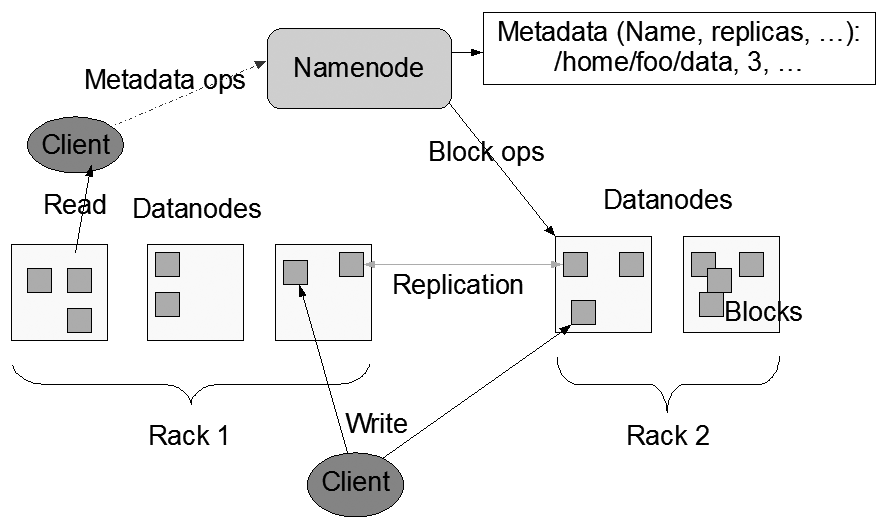
\includegraphics[width=0.8\textwidth]{images/hdfs_architecture.png}
\end{figure}

\subsection{MapReduce}
\label{subsection:mapreduce}

MapReduce~\cite{mapreduce_tutorial} is a software framework, which allows to process vast amounts of data on large clusters. It is reliable and fault-tolerant. A MapReduce job splits the input data into independent chunks. These are first processed in parallel by the map tasks (mappers). With map tasks finished, the framework sorts their output and the results are passed to the reduce tasks (reducers). The framework is responsible for scheduling, monitoring and re-execution of the tasks. In a typical scenario, the MapReduce framework and HDFS are running on the same set of nodes. This configuration allows the framework to effectively schedule the tasks to nodes where the data reside. This way, the system minimizes the amount of network traffic needed for job execution. Similarly to HDFS, also MapReduce has a master/slave architecture. The framework consists of a single master ResourceManager, multiple NodeManagers (one per node of a cluster), and one MRAppMaster per application. The framework application has to specify the input and output locations and supply the implementations for the map and reduce tasks. These and other settings form a job configuration. The process starts when a job client submits a job with a JAR file (Java Archive) or executable to the ResourceManager. The ResourceManager then distributes the software and configuration to the slaves and begins scheduling the tasks. During the execution, it provides status and diagnostic information. 

The framework operates exclusively using \textit{key-value} pairs. It is a fundamental data structure providing users with extensibility. In a key-value based data model the information is stored within collections in which every item is a pair of key and value. Within the framework, the input of a job is a set of key-value pairs. The output of the job is another set of key-value pairs of possibly different types. The classes of keys and values need to be serializable by implementing a dedicated interface. Additionally, the key classes need to be comparable. The standard dataflow of the MapReduce job execution is following:

\begin{enumerate}
	\item The system first divides the input data into splits. These splits have usually 64--128 megabytes (MB). The framework assigns one split to each mapper. Then it begins to read the input data from the HDFS, generating key-value pairs. These pairs are passed to the mappers. In a typical case, if processing plain text files, a key-value pair would be generated for each line in every file located in an input directory.
	
	\item The mapper gets a series of key-value pairs. While processing one input pair it can generate zero or multiple output key-value pairs. The types of input and output keys and values may differ. 
	
	Listing~\ref{listing:wordcount_map} shows an pseudo-code implementation of a map function from the classical WordCount example which performs extraction of word frequencies. In this case the function is called for every line contained in the assigned split. The mapper gets the line and divides it into its words. Then for each of these words it emits an output key-value pair, where key is the word and value is 1. The value represents a single occurrence of the word.

	\item Every output of each mapper is assigned to a specific reducer. The partition function gets the mapper output key and the actual number of reducers and it determines the associated reducer. Then the data are shuffled---they are sorted in parallel, using the provided comparison function, and exchanged between the nodes of mappers and reducers. The performance of this phase is dependent on the speed of the network between cluster nodes.
	
	\item For each unique key, in sorted order, a reducer is called. Reducer iterates over all the values associated with the given unique key. It can generate zero or multiple output key-value pairs. Like in mapper, also in reducer the types of input and output keys or values may differ.
	
	The implementation of a reduce function from the word count example is presented in Listing~\ref{listing:wordcount_reduce}. It sums all the partial counts emitted by mappers into a total count for each of the unique words.
	
	\item Finally, the system stores the output of the reducers to the HDFS. The framework allows the user to define MapReduce batch jobs for executing multiple jobs in a sequence.
\end{enumerate}

\begin{lstlisting}[float=htb!,language=bash,caption={WordCount: map},label={listing:wordcount_map}]
function map(String name, String line):
	for word in line.split():
		emit(word, 1)
\end{lstlisting}

\begin{lstlisting}[float=htb!,language=bash,caption={WordCount: reduce},label={listing:wordcount_reduce}]
function reduce(String word, Iterator partial_counts):
	total_count = 0
	for count in partial_count:
		total_count += count
	emit(word, total_count)
\end{lstlisting}

In order to store and process the July 2015 dataset of the Common Crawl (149 TB, 1.84 billions of pages), we needed a distributed storage and framework for parallel data processing. Therefore, we decided to use the Apache Hadoop for these purposes. When wondering about other means of processing of such a huge dataset, one can get inspired by the list of example projects using Common Crawl data\footnote{\url{http://commoncrawl.org/the-data/examples/} (accessed April 10, 2016)}. One of the examples mentioned in the list is the method described in Chapter~\ref{chapter:related_work}.

\section{WARC-Hadoop}
\label{section:warc_hadoop}

When processing data in a custom format (e.g.\ WARC file format) with Hadoop, the user needs to implement a set of interfaces for the system to handle the data properly. There exist a number of libraries which enable Hadoop to process the WARC files with the MapReduce framework. We decided to utilize one such library, called warc-hadoop~\cite{warc-hadoop} in our experiment.

The warc-hadoop is a Java library providing the functionality for reading and writing WARC files in MapReduce environment. It also enables the framework to serialize and transfer individual WARC records while shuffling the data between the mappers and reducers. This library was created with an intention to help the users explore the content of the Common Crawl datasets.

\section{MetaCentrum}
\label{section:metacentrum}

The Hadoop cluster we use for our experiments is provided by the MetaCentrum\footnote{\url{https://www.metacentrum.cz/en/} (accessed April 10, 2016)} project, which is an activity of the CESNET\footnote{\url{https://www.cesnet.cz/?lang=en} (accessed April 10, 2016)} association. MetaCentrum operates and manages distributed computing infrastructure, which consist of computing and storage resources owned by CESNET and cooperating academic centers located in the Czech Republic. Moreover, MetaCentrum holds responsibility for building the National Grid and its integration with related international activities.

The provided Hadoop cluster in MetaCentrum consists of 3 management nodes and 24 worker nodes. The management nodes run components like front-end, HDFS NameNode and MapReduce History Server. Every node of the configuration has Intel\textregistered{} Xeon\textregistered{} CPU E5-2630 v3 (20 MB Cache, 2.40 GHz) and 128 gigabytes (GB) of memory. The overall disk space available on the cluster is 1.02 petabytes (PB). The HDFS operates with a replication factor of 4, which means that the cluster can hold de facto 261 terabytes (TB) of user data.

Access to computing and storage facilities owned by parties and projects contributing to the National Grid Infrastructure MetaCentrum, provided under the programme "Projects of Large Research, Development, and Innovations Infrastructures" (CESNET LM2015042), is greatly appreciated.

\section{jsoup}
\label{section:jsoup}

Processing data from the web is usually complicated. For example, there are many web pages, that do not have valid HTML structure or are encoded in different character sets. To tackle this we use a library called jsoup~\cite{jsoup}, a Java library for working with real-world HTML structures. It transforms the HTML structure to the Document Object Model (DOM)~\cite{DOM}.

The jsoup library provides a way to extract data using DOM traversal or Cascading Style Sheets (CSS) selectors. Furthermore it allows the user to clean the HTML structure by keeping only the HTML elements and attributes present in a provided whitelist.

In our real-world data experiment, we process Common Crawl dataset with the native Java MapReduce library. Therefore we consider jsoup as suitable library for our needs. We use the library in parallel execution environment to parse the HTML structures of the web pages. The library allows us to scrape the contents of the HTML elements \texttt{<p>} representing paragraphs of text that we consider as input documents to be aligned by our method. We could also collect content of other elements such as \texttt{<h1>}--\texttt{<h6>}, \texttt{<li>}, \texttt{<th>}, \texttt{<td>}, etc., as well.

\section{language-detector}
\label{section:language_detector}

Another Java library we use in our real-world data experiment is language-detector~\cite{language-detector}. As the name suggests, it is a library that performs language detection. It contains built-in profiles for 70 different languages, which were trained using common texts available for each of the languages. The library also allows the user to train a custom language profile when provided with a monolingual corpus. Underneath, the library uses N-gram-based text categorization~\cite{Cavnar94}. 

We use this library while running MapReduce over the Common Crawl dataset. For each of the paragraphs scraped from the web pages, we identify the language using the language-detector library. This way the MapReduce job is able to keep only the paragraphs in the languages of our interest.
